\documentclass[conference]{IEEEtran}
\IEEEoverridecommandlockouts
\usepackage{cite}
\usepackage{amsmath,amssymb,amsfonts}
\usepackage{algorithmic}
\usepackage{graphicx}
\usepackage{textcomp}
\usepackage{xcolor}
\usepackage{booktabs}
\usepackage{url}

\def\BibTeX{{\rm B\kern-.05em{\sc i\kern-.025em b}\kern-.08em
    T\kern-.1667em\lower.7ex\hbox{E}\kern-.125emX}}

\begin{document}

\title{A Hybrid Gradient Boosting Framework for Interpretable Credit Card Fraud Detection}

\author{
\begin{tabular}{cccccc}

\multicolumn{2}{c}{
\begin{tabular}{c}
Bandikolla Rahul \\
\textit{Dept of CSE(AI\&ML)} \\
Vardhaman College of Engineering \\
Hyderabad, India \\
rahulbandikolla@gmail.com
\end{tabular}}
&
\multicolumn{2}{c}{
\begin{tabular}{c}
Bumandla Rajashekar \\
\textit{Dept of CSE(AI\&ML)} \\
Vardhaman College of Engineering \\
Hyderabad, India \\
bumandlarajashekar@gmail.com
\end{tabular}}
&
\multicolumn{2}{c}{
\begin{tabular}{c}
Uppala Vinay \\
\textit{Dept of CSE(AI\&ML)} \\
Vardhaman College of Engineering \\
Hyderabad, India \\
uppalavinay5678@gmail.com
\end{tabular}}
\\[0.6cm]
&
\multicolumn{2}{c}{
\hspace{2.1cm}
\begin{tabular}{c}
Koti Tejasvi\\
\textit{Dept of CSE(AI\&ML)} \\
Vardhaman College of Engineering \\
Hyderabad, India \\
kotitejasvi@gmail.com
\end{tabular}}
&
\multicolumn{2}{c}{
\hspace{1.2cm}
\begin{tabular}{c}
M. A. Jabbar \\
\textit{Dept of CSE(AI\&ML)} \\
Vardhaman College of Engineering \\
Hyderabad, India \\
jabbar.meerja@gmail.com
\end{tabular}}
\end{tabular}
}

\maketitle

\begin{abstract}
Less than a fifth of a percent of credit card transactions in a typical dataset are fraudulent, and that imbalance alone makes reliable detection hard -- on top of it, fraud patterns keep changing as the people committing it adapt to whatever a bank deploys against them. This paper walks through the implementation and evaluation of a complete, end-to-end fraud detection system built around an ensemble of three gradient-boosted tree models: XGBoost, LightGBM, and CatBoost, tuned with Tree-structured Parzen Estimator optimization. The system runs behind a Flask REST API and a React dashboard, and every prediction the dashboard shows comes with a SHAP-based explanation of which features drove it. We describe the full pipeline, report an ensemble PR-AUC of 0.8481 on 5-fold cross-validation and 0.8192 on a stratified 15\% held-out test set never seen during training or hyperparameter selection, and show that the live API reproduces offline scores essentially exactly. We also cover a design path we tried and abandoned: a GraphSAGE-based graph neural network that, once tested properly, turned out to underperform the simpler ensemble -- a result consistent with known heterophily and camouflage effects in fraud transaction graphs. The gap between what the offline experiments predicted and what the deployed API actually returns turned out to be negligible, which is not something every fraud-detection paper checks.
\end{abstract}

\begin{IEEEkeywords}
Fraud Detection, Gradient Boosting, Ensembles, Hyperparameter Optimization, Graph Neural Networks, SHAP
\end{IEEEkeywords}

\section{Introduction}
Digital payments keep growing, and the fraud riding along with them keeps getting harder to catch. Any system meant to catch it has to score huge volumes of high-dimensional transaction data fast, and it has to do that knowing that only a sliver of a percent of what it sees is actually fraud \cite{dalpozzolo2015calibrating, abdallah2016fraud}. Rule-based engines used to be the standard approach; they have mostly been replaced by learned models, and among those, tree-based boosting methods have held up especially well \cite{phua2010comprehensive, bhattacharyya2011data}.

This paper covers the implementation of an ensemble-based fraud detection system, start to finish -- data engineering, hyperparameter search, ensembling, the API that serves it, and the dashboard sitting on top. The core of the system is an average-probability ensemble of XGBoost \cite{chen2016xgboost}, LightGBM \cite{ke2017lightgbm}, and CatBoost \cite{prokhorenkova2018catboost}. Every prediction the dashboard shows a user is accompanied by a SHAP \cite{lundberg2017unified} breakdown of which features pushed the score toward fraud or away from it.

We also document something most papers in this area leave out: a design alternative we built, tested, and rejected. Before settling on the gradient-boosting ensemble, we built a structural Graph Neural Network approach using GraphSAGE \cite{hamilton2017inductive}. It underperformed once we ran the ablation properly, and Section IV covers why, tying the result to the graph heterophily and camouflaged-fraudster literature \cite{zhu2020beyond, dou2020enhancing}.

The rest of the paper is organized as follows. Section II covers related work. Section III walks through the system architecture. Section IV is the graph ablation. Section V is the evaluation, including the deployment validation. Sections VI and VII are discussion, limitations, and conclusion.

\section{Related Work}
Credit card fraud detection via data mining has been surveyed extensively elsewhere \cite{abdallah2016fraud, phua2010comprehensive}, so we won't repeat that ground here. The dataset we use, the European credit card fraud set \cite{dalpozzolo2015calibrating}, shows up throughout this literature specifically because it's a good testbed for imbalance-handling techniques -- SMOTE \cite{macia2011smote} being the most common one applied to it.

XGBoost \cite{chen2016xgboost}, LightGBM \cite{ke2017lightgbm}, and CatBoost \cite{prokhorenkova2018catboost} are, at this point, the default choice for tabular problems in both research and production, mostly because they pick up non-linear feature interactions on their own instead of requiring someone to hand-engineer feature crosses. Tuning them by hand is tedious, though, which is where automated search frameworks like Optuna \cite{akiba2019optuna} come in -- it uses Tree-structured Parzen Estimators \cite{bergstra2011algorithms} under the hood, and it's become close to a standard tool for this kind of work.

Graph Neural Networks are the other thread worth covering. Graph Convolutional Networks \cite{kipf2016semi} and GraphSAGE \cite{hamilton2017inductive} in particular have found use in anomaly detection. There's a catch, though: these architectures generally assume that connected nodes tend to share a label -- homophily. Fraud doesn't cooperate with that assumption. Fraudulent accounts often connect themselves to legitimate ones on purpose, precisely to look less suspicious, and the literature has a name for this: heterophily, or camouflage \cite{zhu2020beyond, dou2020enhancing, liu2021alleviating}. That mismatch is exactly why we ran the comparison in Section IV.

\section{System Architecture}
The system is one pipeline end to end, from raw transaction records to a live dashboard someone can actually click through.

\subsection{Data Pipeline and Feature Engineering}
Training data comes from the Kaggle European credit card fraud dataset -- 28 PCA components ($V1$ through $V28$), plus \textit{Time} and \textit{Amount}, plus the (heavily skewed) \textit{Class} label. Before any modeling happens, the pipeline deduplicates the raw data and derives two engineered features:
\begin{enumerate}
    \item \textbf{Temporal cyclicity}: \textit{Time} gets mapped onto a 24-hour cycle and encoded trigonometrically as $hour\_sin$ and $hour\_cos$, so the model sees "close to midnight" as close regardless of which side of the day boundary a transaction falls on.
    \item \textbf{Magnitude scaling}: \textit{Amount} goes through a $\log(1+x)$ transform ($log1p\_Amount$) to pull in its long tail.
\end{enumerate}
All 33 resulting features get normalized with a scaler \cite{pedregosa2011scikit} fit only on the training folds -- fitting it on anything else would leak test-set statistics into training.

\subsection{Cross-Validation Protocol and Optuna HPO}
Evaluation runs on 5-fold stratified cross-validation. For each model, a single Optuna \cite{akiba2019optuna} study searches hyperparameters against the mean validation PR-AUC across those same five folds -- 76 trials for XGBoost, 55 for LightGBM, and 33 for CatBoost.

\begin{figure}[htbp]
\centerline{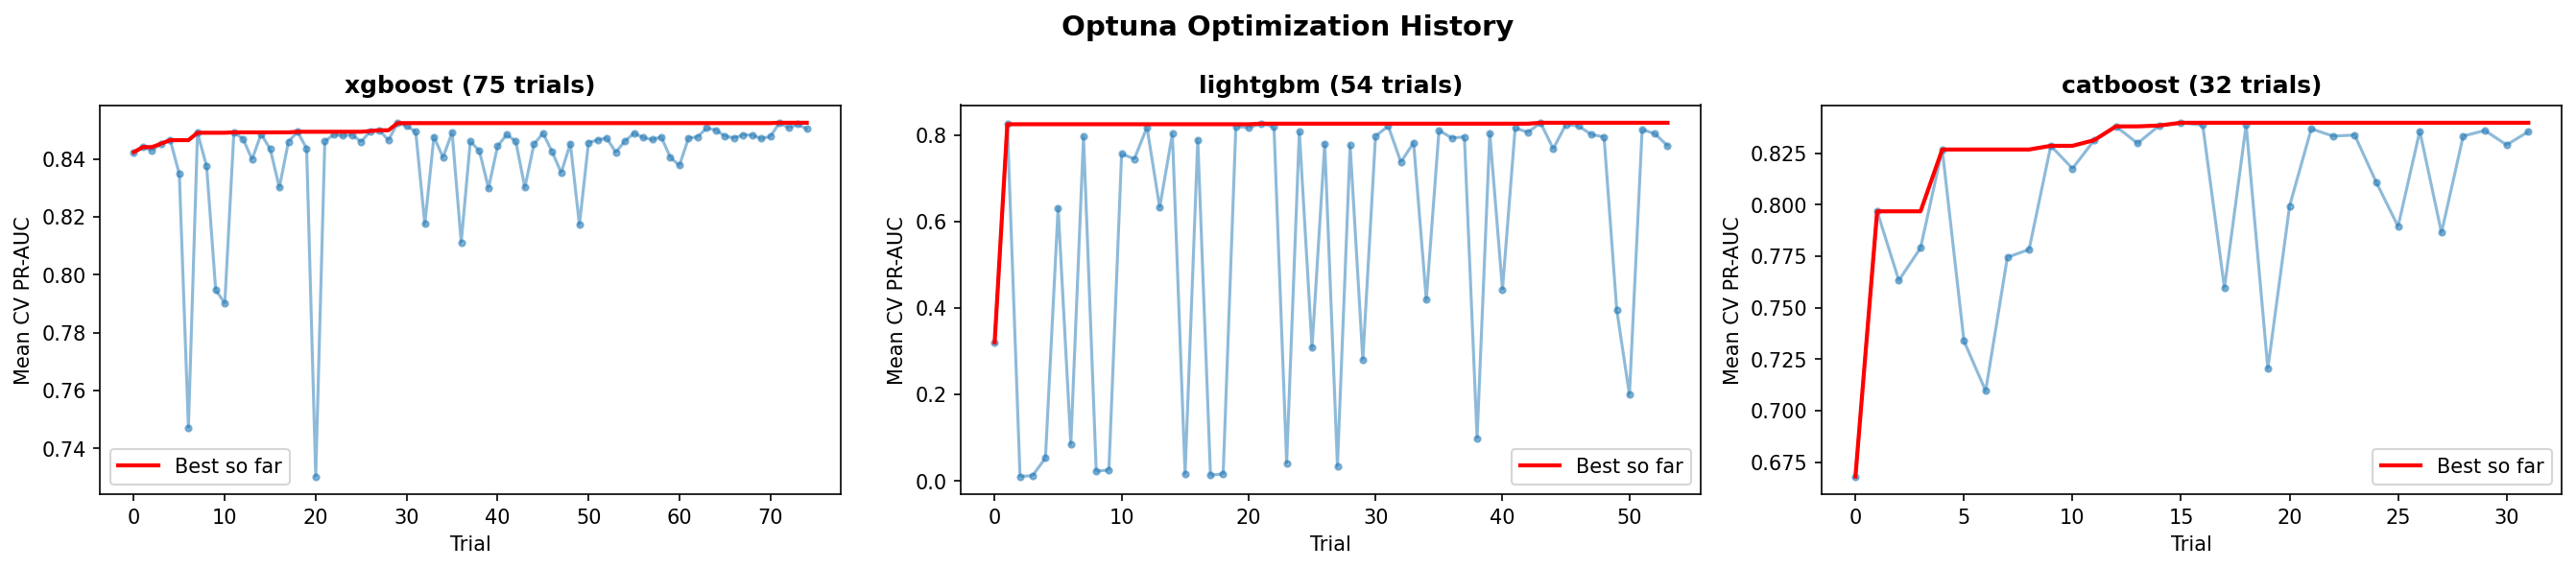
\includegraphics[width=\columnwidth]{figures/optuna_history.png}}
\caption{Optuna search trajectories for all three models. Best-so-far PR-AUC is overlaid on each trial's raw score.}
\label{fig:optuna}
\end{figure}

All three converge quickly, as Fig.~\ref{fig:optuna} shows, though LightGBM's climb out of a weak starting point is the steepest of the three -- its default configuration was genuinely bad, and Section VI gets into why that matters.

\subsection{Ensembling and Model Export}
The deployed model is a simple, unweighted average of the three tuned models' output probabilities: $P = (P_{xgb} + P_{lgb} + P_{cat}) / 3.0$. We picked a decision threshold of 0.7725 by maximizing F1 on out-of-fold predictions. Everything needed to reproduce a prediction outside the notebook -- the fitted scaler, the exact 33-feature column order, and all three tuned models -- gets serialized together for deployment.

\subsection{Flask API and React Dashboard}
A Python Flask \cite{grinberg2018flask} REST API sits behind the dashboard, with three endpoints doing the actual work:
\begin{itemize}
    \item \texttt{/api/predict} -- takes a single transaction, engineers $hour\_sin$, $hour\_cos$, and $log1p\_Amount$ on the fly, forces the 33 columns into the exact order training used, scales them, and returns the ensemble's probability.
    \item \texttt{/api/batch-predict} -- the same thing, but for a whole CSV at once.
    \item \texttt{/api/stats} and \texttt{/api/model-info} -- pull aggregated numbers and metadata straight from the CV summary files, nothing computed on the fly.
\end{itemize}

\begin{figure}[htbp]
\centerline{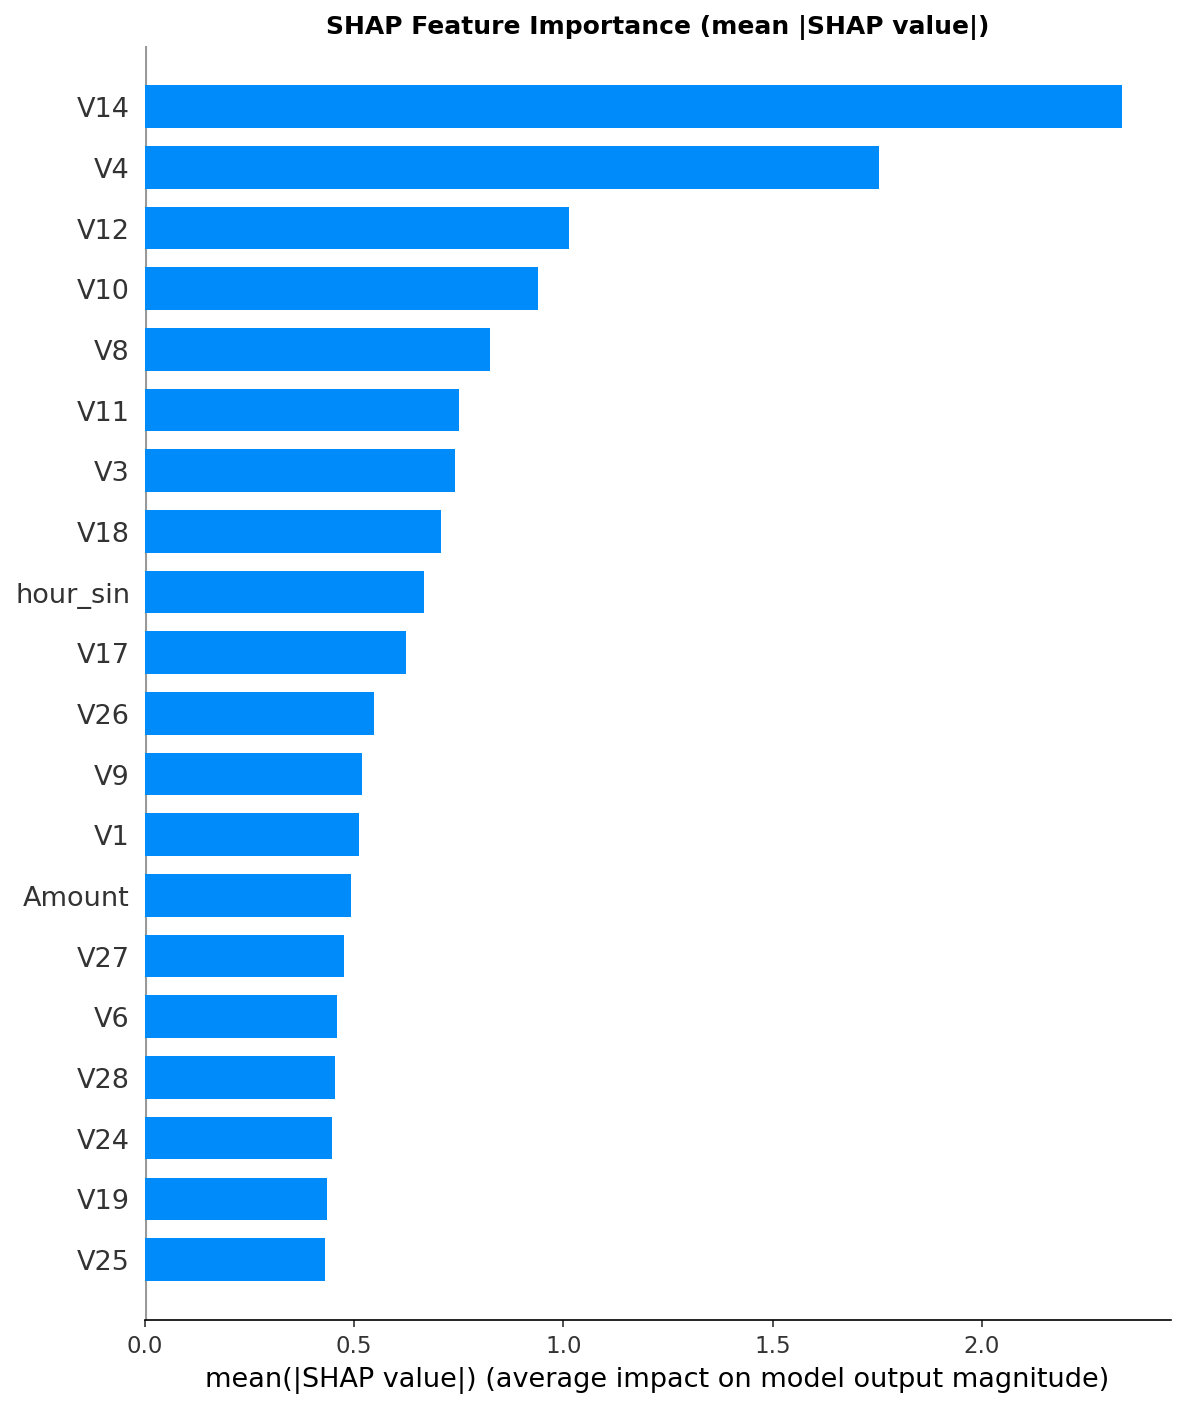
\includegraphics[width=\columnwidth]{figures/shap_importance.png}}
\caption{Global SHAP feature importance for the tuned ensemble (proxied via XGBoost). $V14$, $V4$, and $V12$ lead by a wide margin.}
\label{fig:shap_global}
\end{figure}

On the frontend side, it's a single-page React \cite{facebook2013react} app. A SHAP \texttt{TreeExplainer} \cite{lundberg2017unified} runs inside the API and returns per-transaction feature contributions alongside every prediction, which the dashboard renders as a "Why Flagged" bar chart -- red bars pushing a transaction toward fraud, green ones pulling it back toward genuine.

\begin{figure}[htbp]
\centerline{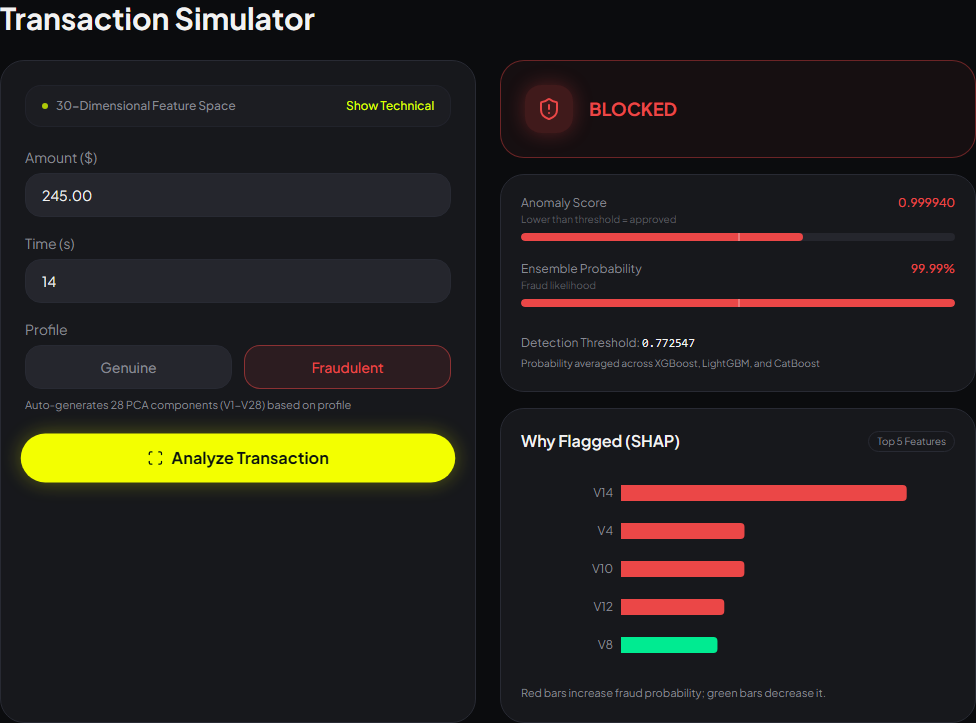
\includegraphics[width=\columnwidth]{figures/dashboard_fraud_view.png}}
\caption{The simulator scoring a fraudulent transaction live. Anomaly score 0.9999 against a threshold of 0.7725 -- the result is a hard BLOCKED classification, not a borderline one.}
\label{fig:dashboard_live}
\end{figure}

\begin{figure}[htbp]
\centerline{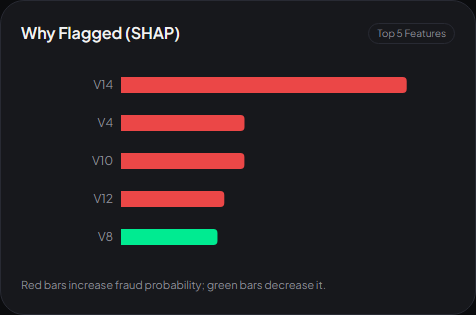
\includegraphics[width=\columnwidth]{figures/shap_fraud_panel.png}}
\caption{The per-transaction explanation for that same fraud case. $V14$, $V4$, $V10$, and $V12$ line up with the global ranking in Fig.~\ref{fig:shap_global}; $V8$ is the one feature pulling in the opposite direction.}
\label{fig:shap_live}
\end{figure}

\section{Graph Ablation Study}
Before settling on the ensemble described above, we built and seriously evaluated a structural graph approach -- internally, we just called it "FraudGuard." The idea was to treat transactions as nodes in a k-Nearest Neighbors graph, run GraphSAGE over that graph to get structure-aware embeddings, and feed those embeddings into an Autoencoder trained to flag anomalies by reconstruction error.

The question we actually needed answered was narrower than "does this work": did the GraphSAGE aggregation step add anything over a plain Autoencoder running on the same tabular features with no graph at all? We compared the full FraudGuard pipeline against that ablated PlainAE baseline across 5 cross-validation splits to find out.

\begin{figure}[htbp]
\centerline{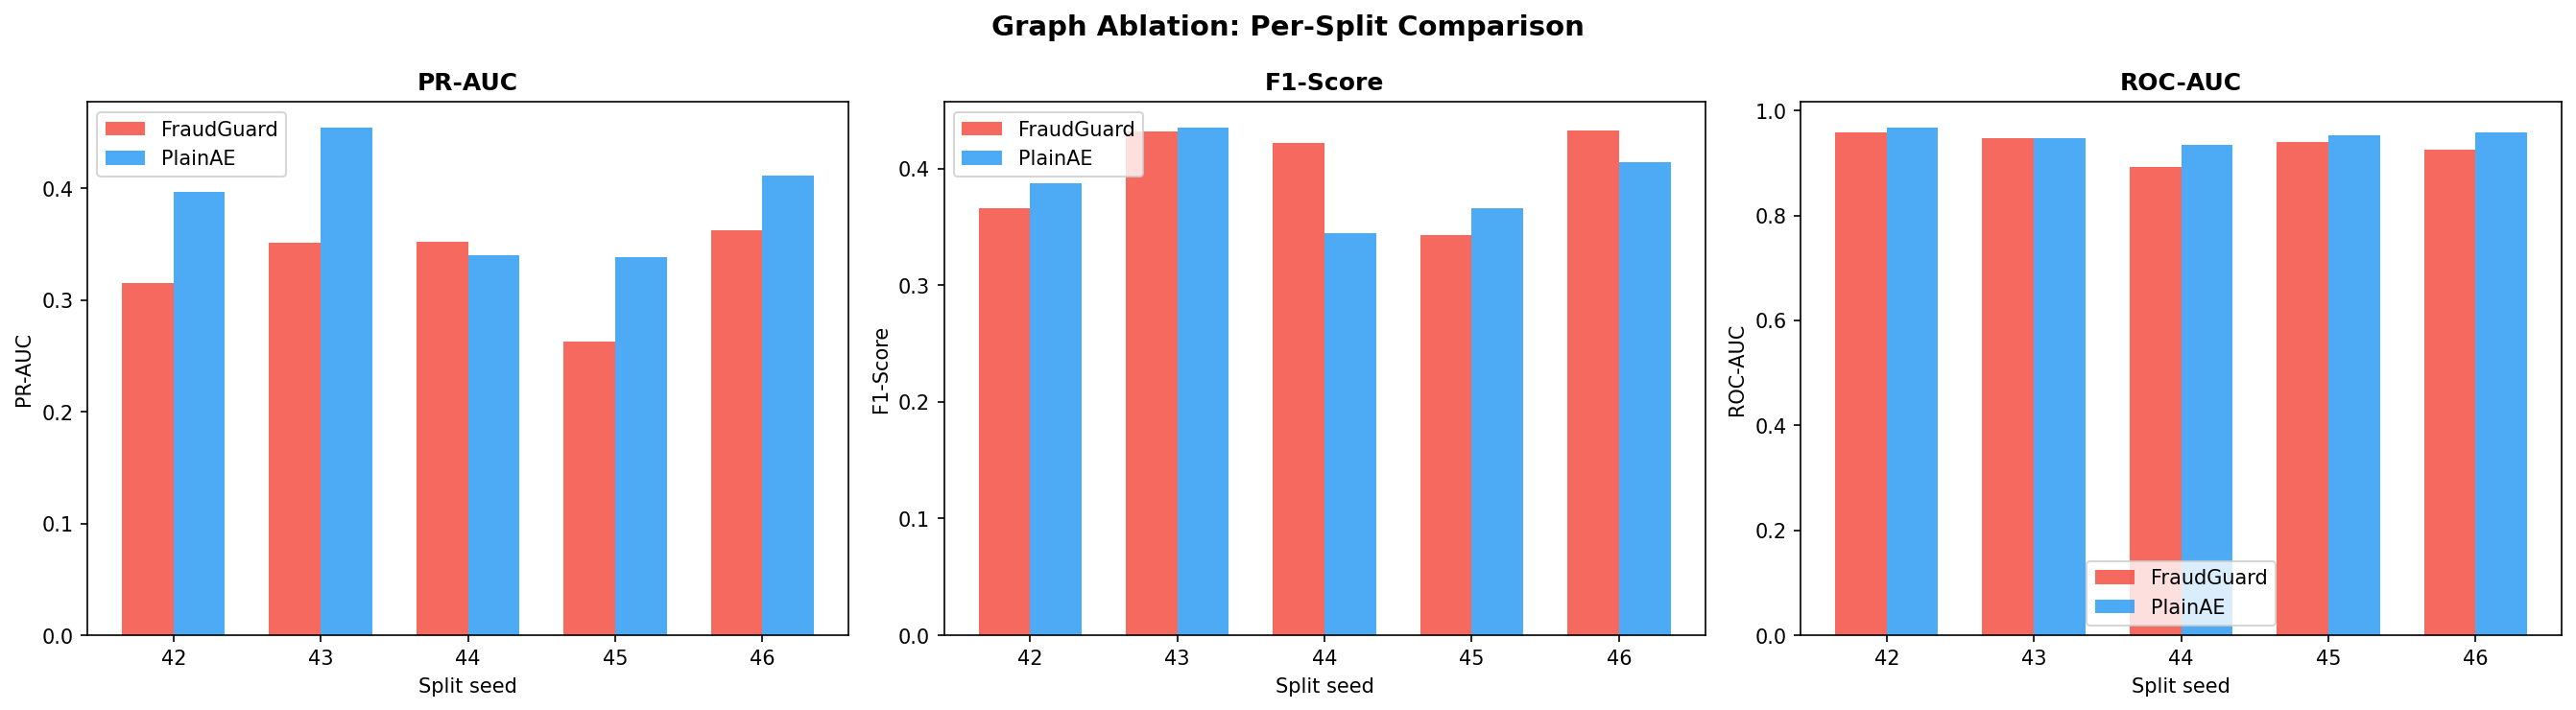
\includegraphics[width=\columnwidth]{figures/graph_ablation_comparison.png}}
\caption{FraudGuard against the ablated Autoencoder, split by split. PR-AUC and ROC-AUC both come out lower with the graph component included.}
\label{fig:ablation_comp}
\end{figure}

\begin{figure}[htbp]
\centerline{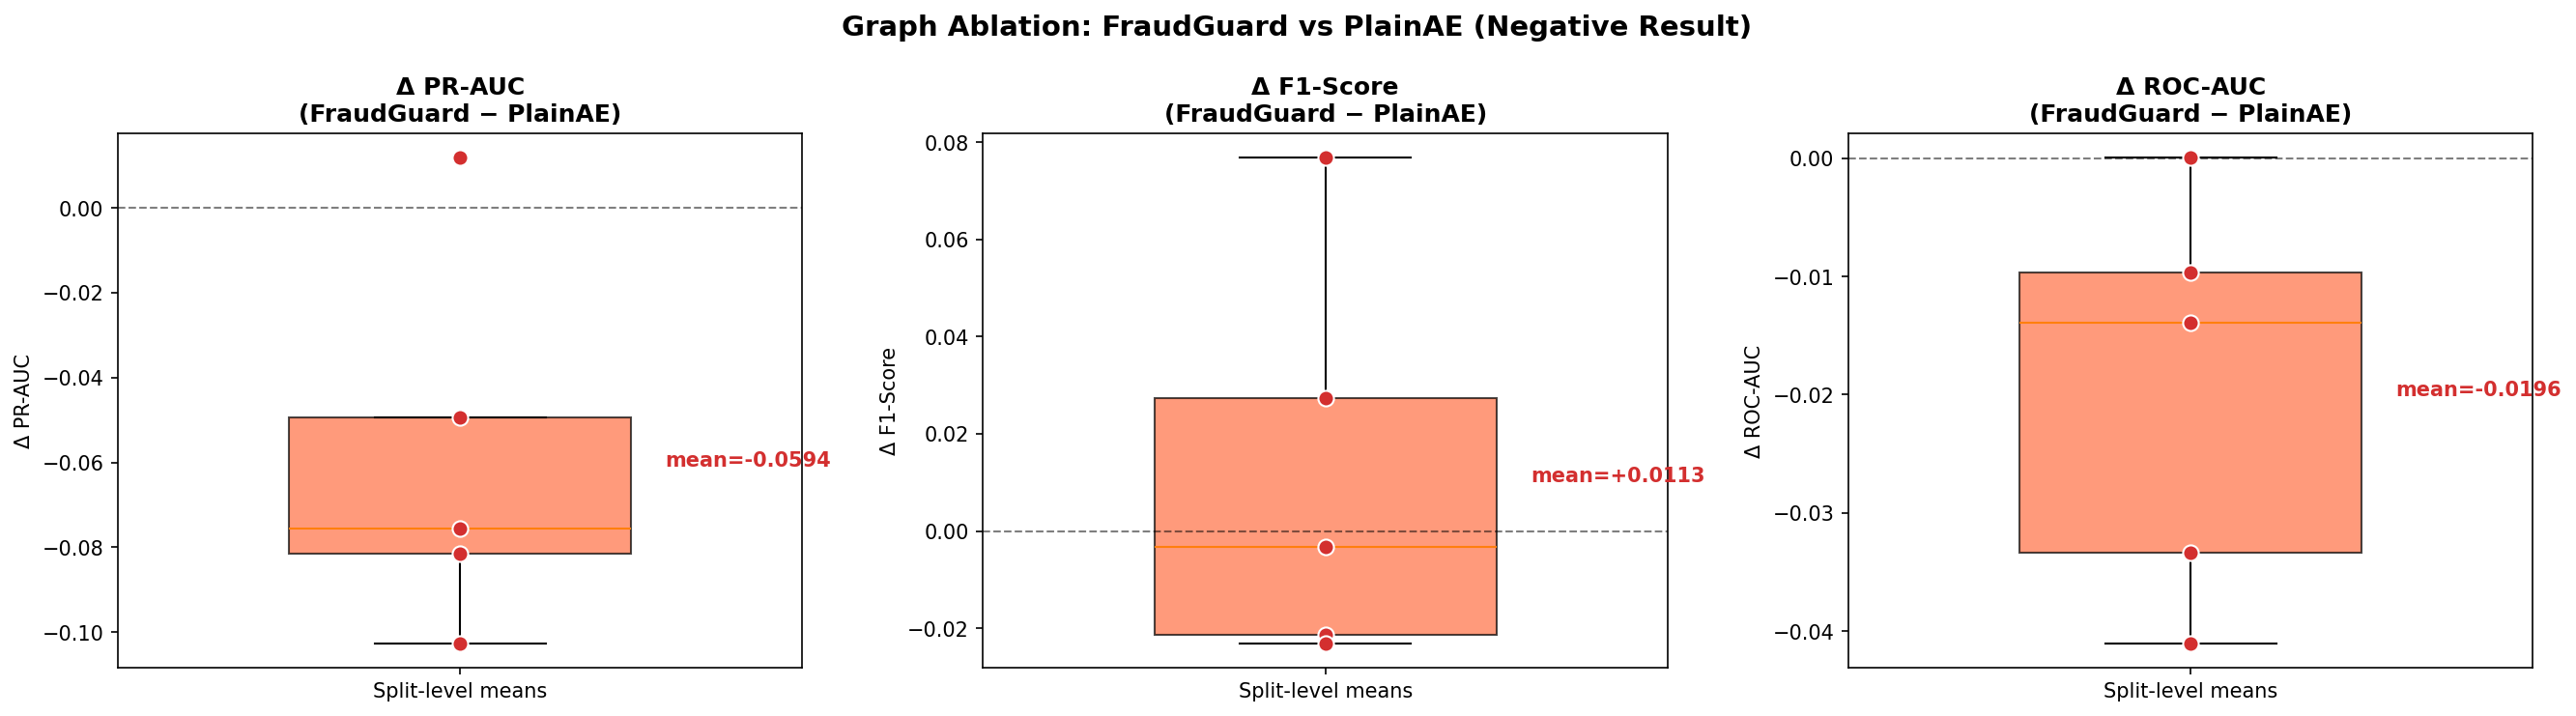
\includegraphics[width=\columnwidth]{figures/graph_ablation_deltas.png}}
\caption{Per-split deltas, FraudGuard minus PlainAE. Everything below zero means the graph made things worse on that split.}
\label{fig:ablation_deltas}
\end{figure}

The answer was no -- worse than no, actually. FraudGuard's mean PR-AUC came in at 0.3285 ($\pm 0.0411$) against PlainAE's 0.3879 ($\pm 0.0495$), a delta of $-0.0594$ with Cohen's $d = -1.345$. ROC-AUC told the same story: $-0.0195$, $d = -1.146$. Figs.~\ref{fig:ablation_comp} and~\ref{fig:ablation_deltas} lay this out split by split, and it's consistent, not a fluke on one partition.

This isn't a surprising result once you look at what's known about GNNs in adversarial settings. GraphSAGE and similar message-passing methods assume nearby nodes look alike; fraud actively works against that by camouflaging itself among legitimate transactions, and the aggregation step ends up smoothing away exactly the signal it was supposed to sharpen \cite{dou2020enhancing, liu2021alleviating}. We dropped the graph component and moved forward with the plain tabular ensemble.

\section{Evaluation}

\subsection{Cross-Validation Results}
Fig.~\ref{fig:cv_results} lays out how each tuned model performed against the final ensemble, averaged across the same 5 CV folds used everywhere else in this paper.

\begin{figure}[htbp]
\centerline{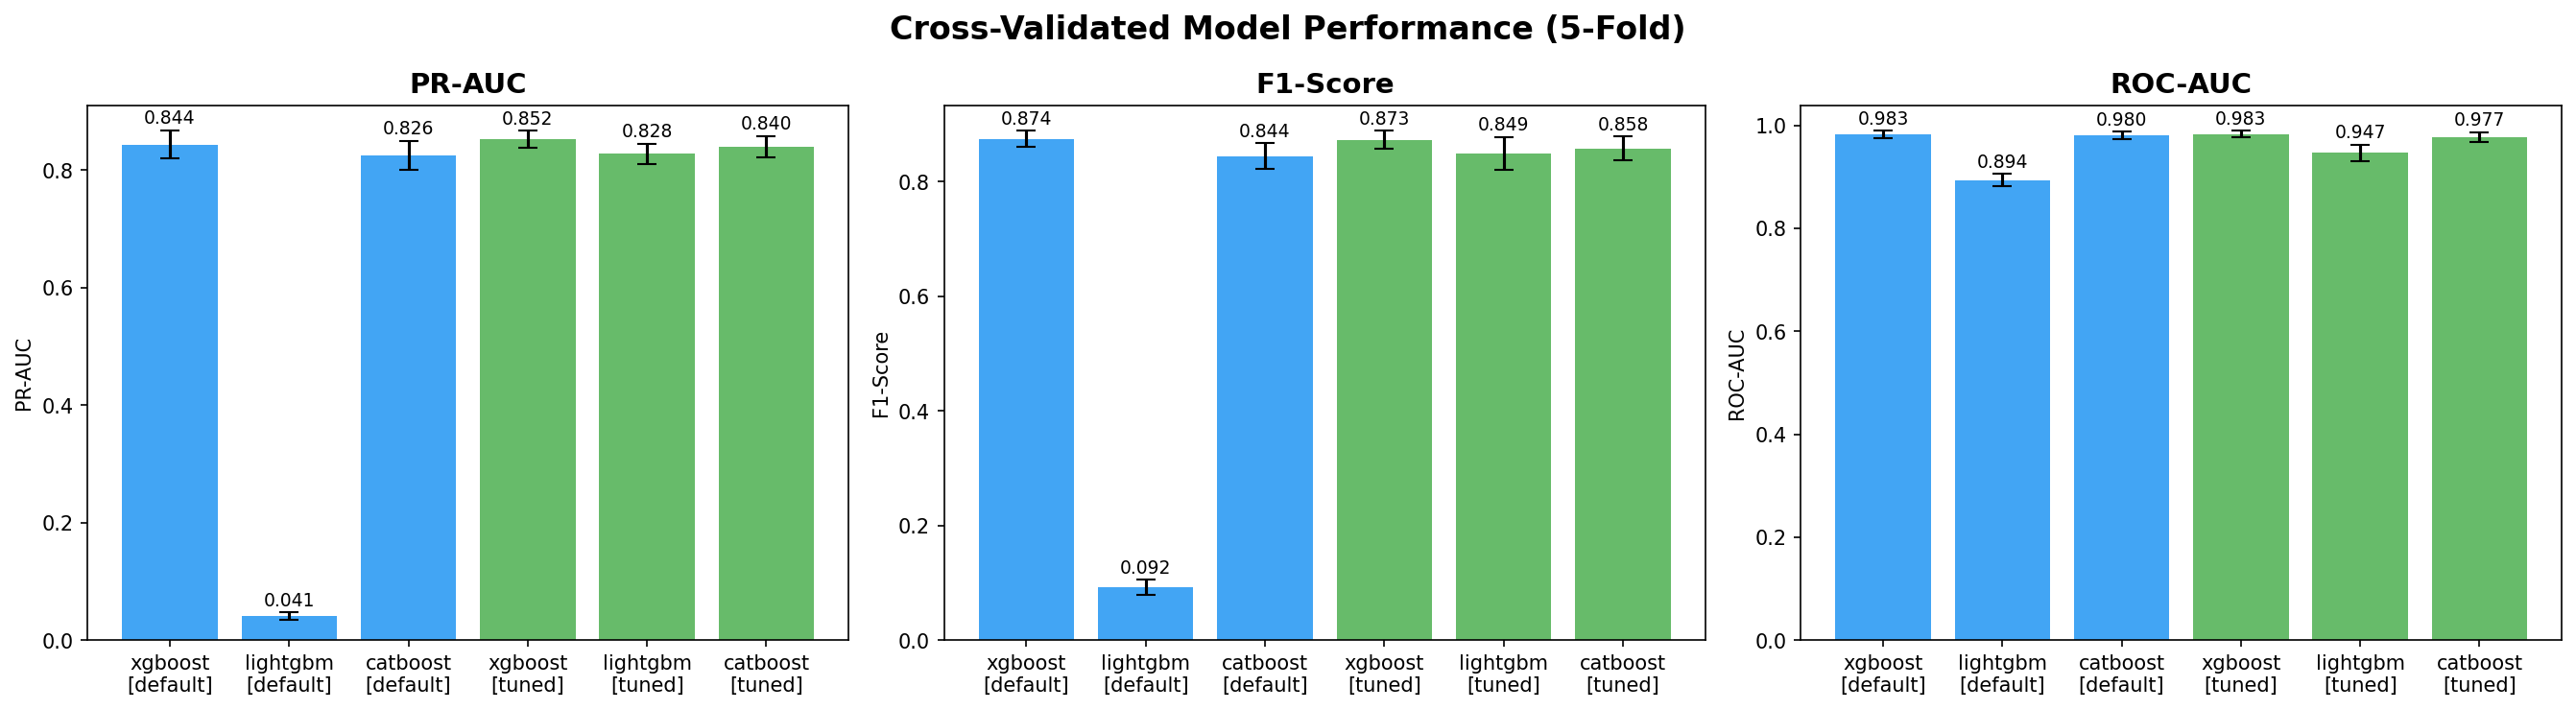
\includegraphics[width=\columnwidth]{figures/cv_results_barplot.png}}
\caption{PR-AUC, F1, and ROC-AUC for every model at both default and tuned settings, plus the ensemble. LightGBM's default-to-tuned jump is the largest by a wide margin.}
\label{fig:cv_results}
\end{figure}

The ensemble lands at 0.8481 PR-AUC, 0.8600 F1, 0.9799 ROC-AUC -- 384 true positives, 36 false positives, 89 false negatives. Averaging the three models' probabilities together mostly buys variance reduction: no single model's idiosyncrasies dominate the final score.

\subsection{Explainability}
Fig.~\ref{fig:shap_beeswarm} is the global view of what the SHAP values look like across the whole feature set. $V14$, $V4$, and $V12$ are doing most of the work, unsurprisingly, but $hour\_sin$ -- the engineered feature -- cracks the top 10, which is a decent sign that the temporal-cyclicity step in Section III-A was worth adding rather than just extra complexity.

\begin{figure}[htbp]
\centerline{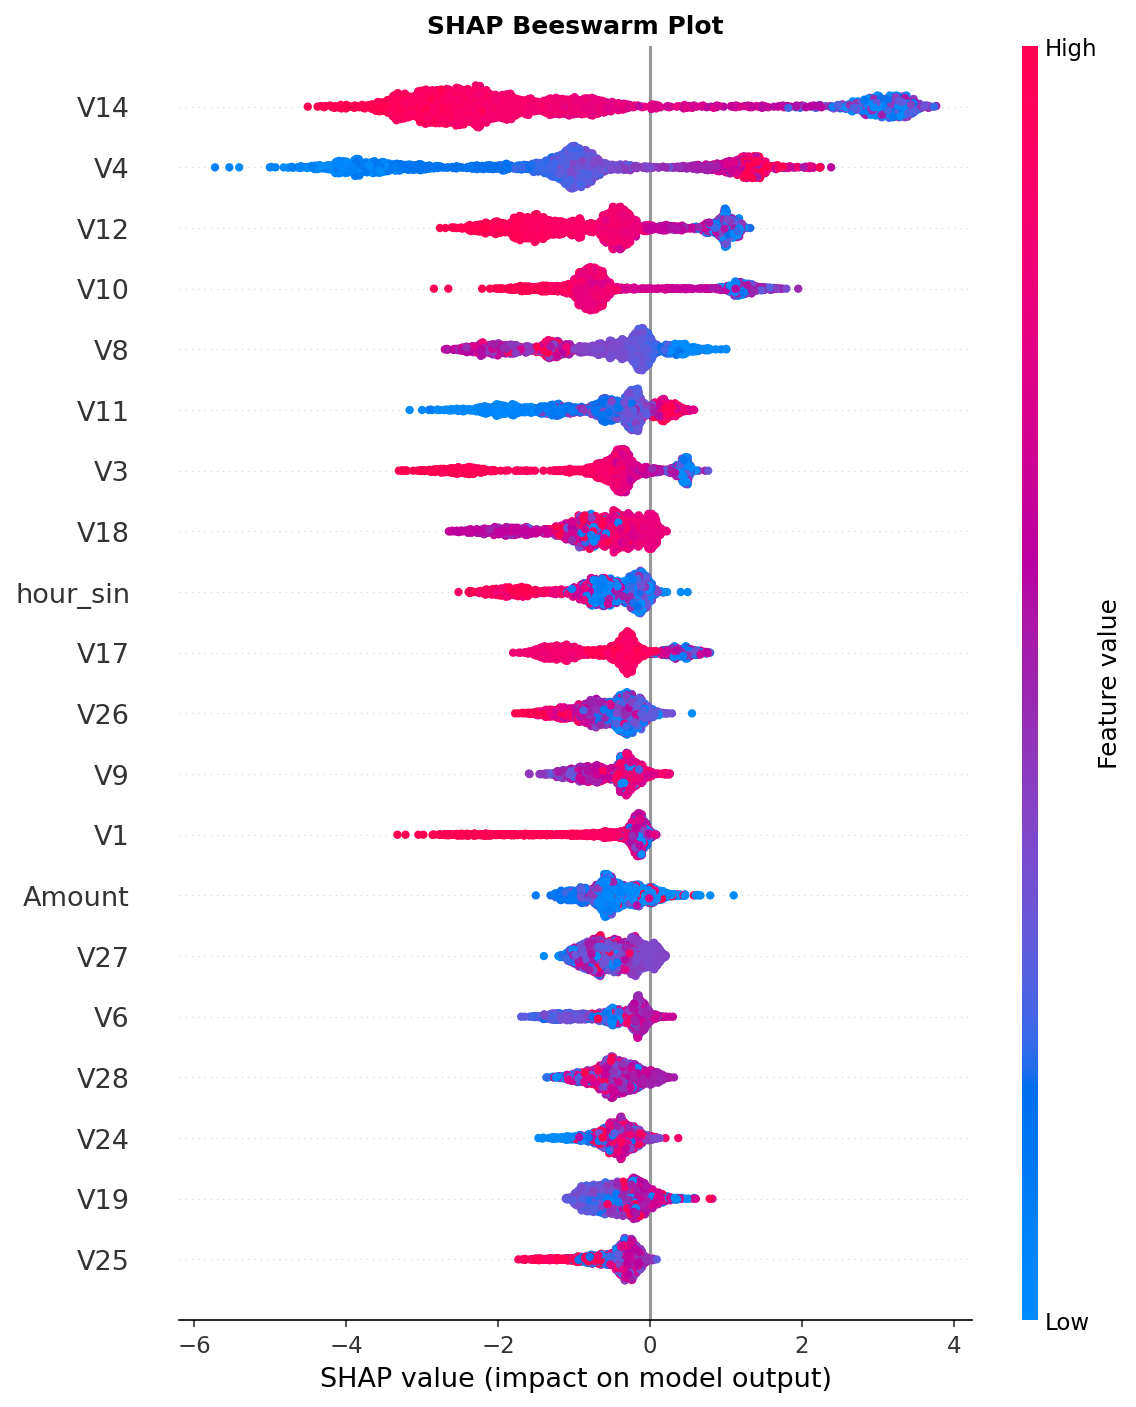
\includegraphics[width=\columnwidth]{figures/shap_beeswarm.png}}
\caption{SHAP beeswarm across the full feature set. High $V4$ pushes toward fraud; high $V14$ pushes the other way.}
\label{fig:shap_beeswarm}
\end{figure}

\subsection{Deployment Validation}
One of the more common ways an ML system quietly breaks in production is a mismatch between what the offline pipeline does and what the deployed API actually does -- a scaler fit differently, columns in a different order, a feature computed at the wrong point in the pipeline. We checked for exactly that: 10 transactions (5 fraud, 5 genuine), scored two ways -- once directly in Python against the serialized offline models, and once by sending the identical raw features to the live \texttt{/api/predict} endpoint over HTTP.

\begin{table}[htbp]
\caption{Deployment Sanity Check: Offline vs. API Scores}\label{tab:sanity_check}
\begin{center}
\begin{tabular}{llccc}
\toprule
\textbf{Id} & \textbf{True Class} & \textbf{Offline Score} & \textbf{Online API Score} & \textbf{Delta ($\Delta$)} \\
\midrule
0 & Fraudulent & 0.9999030 & 0.9999030 & 7e-08 \\
1 & Fraudulent & 0.9745024 & 0.9745024 & 4e-07 \\
2 & Fraudulent & 0.9998607 & 0.9998607 & 2e-07 \\
3 & Fraudulent & 0.9998690 & 0.9998690 & 7e-08 \\
4 & Fraudulent & 0.9999244 & 0.9999244 & 4e-07 \\
5 & Genuine    & 0.0000168 & 0.0000168 & 1e-07 \\
6 & Genuine    & 0.0000134 & 0.0000134 & 4e-07 \\
7 & Genuine    & 0.0000540 & 0.0000540 & 6e-08 \\
8 & Genuine    & 0.0000251 & 0.0000251 & 1e-07 \\
9 & Genuine    & 0.0000311 & 0.0000311 & 1e-07 \\
\bottomrule
\end{tabular}

\end{center}
\end{table}

All 10 matched, with deltas in the $10^{-7}$ range -- floating-point noise, nothing more. That tells us the feature engineering and column ordering are happening in the same sequence in both places, and that the live model is seeing the same 33-column array the offline pipeline saw. It's worth being upfront about the limit here, though: none of these 10 rows sit near the 0.7725 threshold, so this checks pipeline fidelity, not necessarily behavior at the decision boundary specifically.

\subsection{Held-Out Test Set Validation}
The cross-validation metrics reported above were computed on the same folds used to select hyperparameters -- a source of mild optimistic bias acknowledged in Section~VI. To get a number that isn't touched by that bias at all, we carved out a stratified 15\% holdout (42,559 transactions, 71 fraudulent) held aside from training and hyperparameter selection entirely. The three models were retrained once on the remaining 85\% using the same tuned hyperparameters already selected by Optuna, with a fresh scaler fit only on the development set, and scored on the holdout with the same ensemble averaging and 0.7725 threshold.

\begin{table}[htbp]
\caption{Held-Out Test Set Results (Ensemble, $n=42{,}559$)}\label{tab:holdout}
\begin{center}
\begin{tabular}{lc}
\toprule
\textbf{Metric} & \textbf{Value} \\
\midrule
PR-AUC   & 0.8192 \\
F1       & 0.8527 \\
ROC-AUC  & 0.9669 \\
Precision & 0.9483 \\
Recall    & 0.7746 \\
\midrule
TP / FP / TN / FN & 55 / 3 / 42{,}485 / 16 \\
\bottomrule
\end{tabular}

\end{center}
\end{table}

The holdout PR-AUC of 0.8192 (Table~\ref{tab:holdout}) sits about 0.03 below the CV figure of 0.8481, which is roughly what you'd expect given the fold-overlap bias discussed in Section~VI. The drop is real but modest -- the system isn't dramatically overfitting to the CV folds, it's just getting a small free ride from having seen the same partitions during both tuning and evaluation. The holdout F1 (0.8527) and ROC-AUC (0.9669) tell the same story: slightly lower than CV, but in the same ballpark.

\section{Discussion and Limitations}
The clearest lesson from this project is how much hyperparameter tuning can matter, and how unevenly it matters across models. LightGBM's default configuration was close to useless on this data -- PR-AUC of 0.0407 -- and TPE tuning brought it up to 0.8281, the single largest jump in the whole comparison (Fig.~\ref{fig:cv_results}).

The ensemble itself is a mixed story, and we'd rather say that plainly than oversell it. A paired Wilcoxon signed-rank test across the 5 CV folds -- the same method used for the graph ablation in Section~IV -- gives a mean PR-AUC delta of $-0.0035$ (ensemble minus XGBoost), Cohen's $d = -0.638$, and $p = 0.3125$. XGBoost wins on 4 of the 5 folds, and the graduated-verdict rule flags this as ``tends to degrade.'' In plain terms: the ensemble doesn't improve on the best single model by PR-AUC, and if anything it sits slightly below it. What the ensemble buys instead of raw accuracy is variance reduction -- it's less likely to fail badly on the specific edge cases any one of the three models handles poorly, even if its average-case PR-AUC is a fraction of a point worse.

One limitation worth flagging directly: hyperparameters were chosen by maximizing performance on the same five folds we then used to report the CV metrics in Section~V-A. That's a real source of mild optimistic bias, and the held-out results in Section~V-D (PR-AUC 0.8192 vs.\ the CV's 0.8481) confirm it -- the gap is modest but real. The held-out evaluation addresses this limitation for the purposes of reporting an unbiased generalization estimate, though a fully nested cross-validation protocol would be the more rigorous long-term fix. A second limitation: for latency reasons, the live SHAP explanations come from XGBoost alone, used as a stand-in for the full ensemble. Gradient-boosted models tend to agree on decision boundaries in broad strokes, but there will be edge cases where LightGBM or CatBoost is actually driving the score and XGBoost's explanation doesn't quite match what's really happening.

\section{Conclusion}
We built and deployed a fraud detection system around an XGBoost/LightGBM/CatBoost ensemble, and along the way we tested -- and rejected -- a graph-based alternative once the numbers showed it degrading performance under exactly the heterophily and camouflage conditions the literature predicts for this kind of data. The deployment validation confirms the live API isn't just close to the offline numbers, it reproduces them to floating-point precision. The system achieves a CV PR-AUC of 0.8481 and a held-out PR-AUC of 0.8192 on data never seen during training or hyperparameter selection, and gives a SHAP-based explanation for every transaction it scores.

\bibliographystyle{IEEEtran}
\bibliography{references}

\end{document}